\chapter{Conclusions and Future Work}
\label{chp:future_work}

In this preceding chapters, we described structures that help models be more adaptive at the three different stages of their lifecycle.
Specifically, we used implicit and explicit structures along with \textit{adversarial testing}, \textit{runtime monitoring}, and \textit{domain adaptation} to build more adaptive machine learning systems.
We now describe some directions for extending these techniques for future work.


\section{Large Scale Structure-aware Authorship Attribution}
\label{sec:future_work:scale}
In this extension, the goal is to test the generalizability of our findings related to the improvements offered by utilizing forum graph structures on the darkweb (Chapter~\ref{chp:sysml}).
Recent work on cross-domain authorship attribution using text has determined that certain domains (eg. Reddit) are more useful for training authorship attribution models that generalize to other domains~\cite{barlas2020cross,riverastao2021learning}.
Specifically, \citet{riverastao2021learning} demonstrate that in the source domain, diversity in the expressed topics and larger number of unique users play a role in explaining better transfer to target domains.
However, this work does not utilize the additional structure and context present in different domains.
We posit that these graphs can provide information orthogonal to that which is already present in the text.
In this direction of future work, we aim to demonstrate that even in scenarios with an abundance of text/users (over 100k users/1M text posts), these graph structures help improve authorship identification within a single domain, and also help better generalize across domains.
Chapter~\ref{chp:sysml} shows that this is true in the complementary setting with fewer users ($\approx$ 1-10k)
In the remainder of this section, we first describe the choices that are involved in constructing graph structures and their similarities across domains. 
We then describe some preliminary work on utilizing these structures for authorship attribution on Reddit and share our preliminary findings.
To conclude this section, we describe additional directions that we hope to explore, including the associated datasets and techniques. % that help with \textit{domain generalization}.

\subsection{Graphs in Authorship Attribution}

Prior to the prevalence of neural network approaches, seminal work in computational authorship attribution~\cite{stamatatos2009survey} often used syntax-based features including, part-of-speech tags, phrase structures, and syntactic error-based features, among others.
These features may also improve neural authorship attribution models but are not the graphs focal to our analysis.
Instead, we center our work on online content platforms and identify the organizational structures that they use.
A multitude of platforms that involve individuals posting content online have associated graph structures.
We focus on structures common to platforms that face potential challenges with content moderation where authorship identification has the potential to play an important role.
%Figure~\ref*{fig:future_work:scale:graphs:ocp} demonstrates that 
While individual platforms may differ, there exists a shared, underlying, meta-structure, which can be used to identify patterns that aid in stylometric analyses across domains.
In Figure~\ref{fig:future_work:scale:preliminary:reddit_meta} we show a metagraph for a specific platform but note that the the thread-comment-user structure is shared across other platforms as well.
Additional nodes in the metagraph are specific to the platform of interest.
In the following section, we focus on a specific platform - Reddit - and utilize its structure to provide preliminary evidence for its potential.

\begin{comment}
\begin{figure}
    \centering
    \begin{subfigure}{0.48\linewidth}
    \centering
        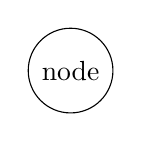
\begin{tikzpicture}[main/.style = {draw, circle}] 
            \node[main] (1) {node};
        \end{tikzpicture}    
    \end{subfigure}
    \begin{subfigure}{0.48\linewidth}
        \centering
        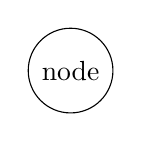
\begin{tikzpicture}[main/.style = {draw, circle}] 
            \node[main] (1) {node};
        \end{tikzpicture}
    \end{subfigure}
    \begin{subfigure}{0.48\linewidth}
        \centering
        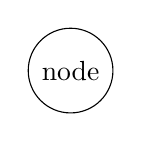
\begin{tikzpicture}[main/.style = {draw, circle}] 
            \node[main] (1) {node};
        \end{tikzpicture}
    \end{subfigure}
    \caption{Example of shared meta-structure in graph structures on Online Content Platforms}
    \label{fig:future_work:scale:graphs:ocp}
\end{figure}
\end{comment}

\subsection{Preliminary Analysis: Reddit Graph-aware Authorship Identification}

\subsubsection{Dataset}
\begin{figure}
    \begin{subfigure}{0.34\linewidth}
        \centering
        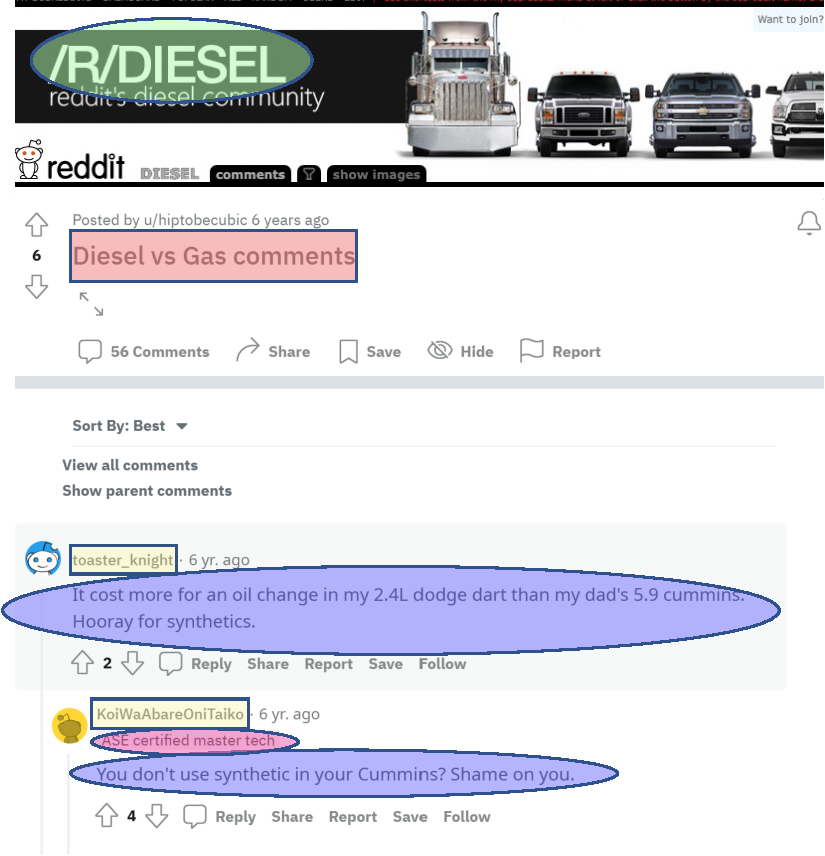
\includegraphics[width=\linewidth,alt={Reddit Metagraph.}]{future_work/figures/reddit_metagraph.pdf}
    \end{subfigure}
    \begin{subfigure}{0.64\linewidth}
        \resizebox{\linewidth}{!}{
         \begin{tikzpicture}
            \node [ellipse,fill=green!30,line width=1.5mm] (subreddit) {Subreddit};
            \node [rectangle,fill=red!40, line width=1.5mm, below right=1cm of subreddit] (thread) {Thread};
            \node [ellipse, fill=blue!50, below right=1cm of thread] (comment) {Comment};
            \node [rectangle, fill=yellow!30,below left=0.5cm and 3cm of comment] (user) {User};
            \node [ellipse, fill=cb-rose,above left = 1cm of user] (flair) {User Flair};
            \draw[thick,<->] (subreddit) -- (thread);
            \draw[thick,<->] (thread) to[bend right] (comment);
            \draw[thick,->] (thread) to[bend left] node[fill=white] {child} (comment);
            \draw[thick,->] (comment) to[loop right] node {child} (comment);
            \draw[thick,<->] (comment) to[bend left] (user);
            \draw[thick,<->] (user) -- (flair);
            \draw[thick,<->] (flair) -- (subreddit);
        \end{tikzpicture}
        }
    \end{subfigure}
    \centering
    \caption{Metagraph of Reddit used for preliminary analysis.}
    \label{fig:future_work:scale:preliminary:reddit_meta}
\end{figure}
We collected data from a snapshot of Reddit comments over one month (Aug 2016) from the collection released by \citet{baumgartner2020pushshift}.
Figure~\ref*{fig:future_work:scale:preliminary:reddit_meta} describes the metagraph corresponding to the graph that we construct from this snapshot.
We use directed edges to distinguish comments that are direct descendants of the parent comment/thread. 
Note that the raw data collected includes only the comments posted within the month; thus, for certain comments, the text corresponding to the direct parent thread/comment may be unavailable as they are posted in the previous month. 
These comments could lead to disconnected components in the graph.
To ensure that the graph is connected, we add a bidirectional edge from each comment to the thread where it was posted.
Table~\ref*{tab:future_work:scale:preliminary:reddit_stats} shows summary statistics about the graph constructed for this dataset.

\begin{table}
    \centering
    \begin{tabular}{cc}
        \toprule
        Entity & Approximate Count \\
        \midrule 
        Subreddits &  $63,000$ \\
        Authors & $3,250,000$ \\
        Comments & $70,000,000$ \\
        Nodes & $79,100,000$ \\
        Edges & $300,000,000$\\
        \bottomrule
    \end{tabular}
    \caption{Dataset used for preliminary analysis of graphs for authorship attribution on Reddit.}
    \label{tab:future_work:scale:preliminary:reddit_stats}
\end{table}

\subsubsection{Goals}
We aim to evaluate our proposed approaches for author identification in a retrieval based setup commonly used in this setting in prior work~\cite{andrews2019learning,riverastao2021learning,khan2021deep,maneriker2021sysml}.
That is, we get a sample query text(s) and must retrieve the nearest author from a collection of target texts.
The query and target texts that the methods are evaluated on are each collected from a different time periods compared to the training set.
This ensures that the embeddings for specific authors are robust to temporal shifts.
Ensuring this is particularly challenging in the graph setting as there are multiple mechanisms to construct graphs across different time periods.
There may be authors who post in both the training, test query, and test target time periods.
In chapter~\ref{chp:sysml}, we describe one strategy where we only use subforum embeddings.
While they do provides improvements (Sec~\ref{sec:sysml:eval}), here we propose alternative mechanisms to incorporate further structural information.
It is not possible to connect the graphs across different time periods as using the same node to denote the author in disjoint time periods would lead to a trivial embedding solution (unique node embedding for the author).
One strategy to deal with the temporal challenge is to use separate graphs for the training and testing time periods, aligning node embeddings across them.
This corresponds to the vertex nomination problem across multiple graphs, and strategies include using orthogonal procrustes~\cite{agterberg2020vertex}) for alignment.
Alternatively, node attributes such as text, time, and label could be used to construct heterogeneous, attributed graphs.
In the latter construction, certain inductive representation learning techniques for large graphs may be applied~\cite{hamilton2017inductive,xu2020inductive}.
We will now describe our initial explorations with these approaches and follow with potential future directions.

\subsubsection{Methods}
%We investigate two preliminary approaches to use the graph corresponding to the metagraph provided in Figure~\ref{fig:future_work:scale:preliminary:reddit_meta}.
\textbf{Structure-based}

\begin{figure}
    \centering
    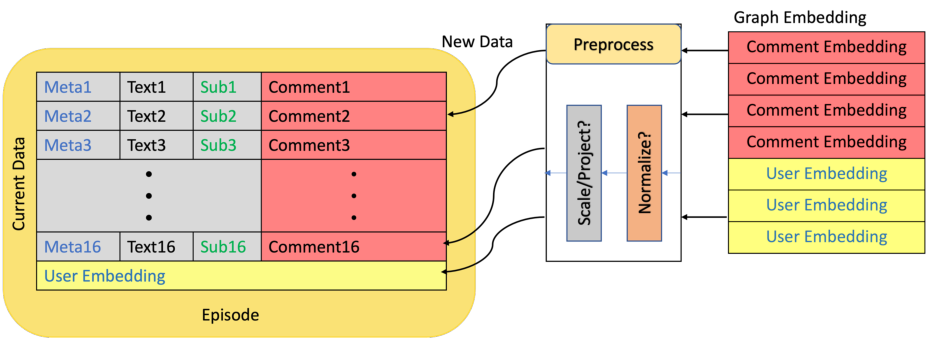
\includegraphics[width=0.9\linewidth,alt={Block diagram of structure-based approach.}]{future_work/figures/reddit_structure_based.pdf}
    \caption{Structure-based Author Identification Embedding}
    \label{fig:future_work:scale:preliminary:reddit_structure_embedding}
\end{figure}
In the first approach, which we designate as the \textit{structure-based} approach, we use separately generate embeddings from the structure of the Reddit graph, use a separate neural network to embed text/metadata in each episode, and then fuse the two embeddings to generate a structure-aware embedding. 
The graph embedding may need to be transformed/scaled before it is combined with the embeddings of non-graph features to ensure that their magnitudes are comparable.
Thus, we transform the embeddings prior to fusing them.
Figure~\ref{fig:future_work:scale:preliminary:reddit_structure_embedding} demonstrates the structure-based embedding approach for author identification.

\textbf{Context-based}
\begin{figure}
    \centering
    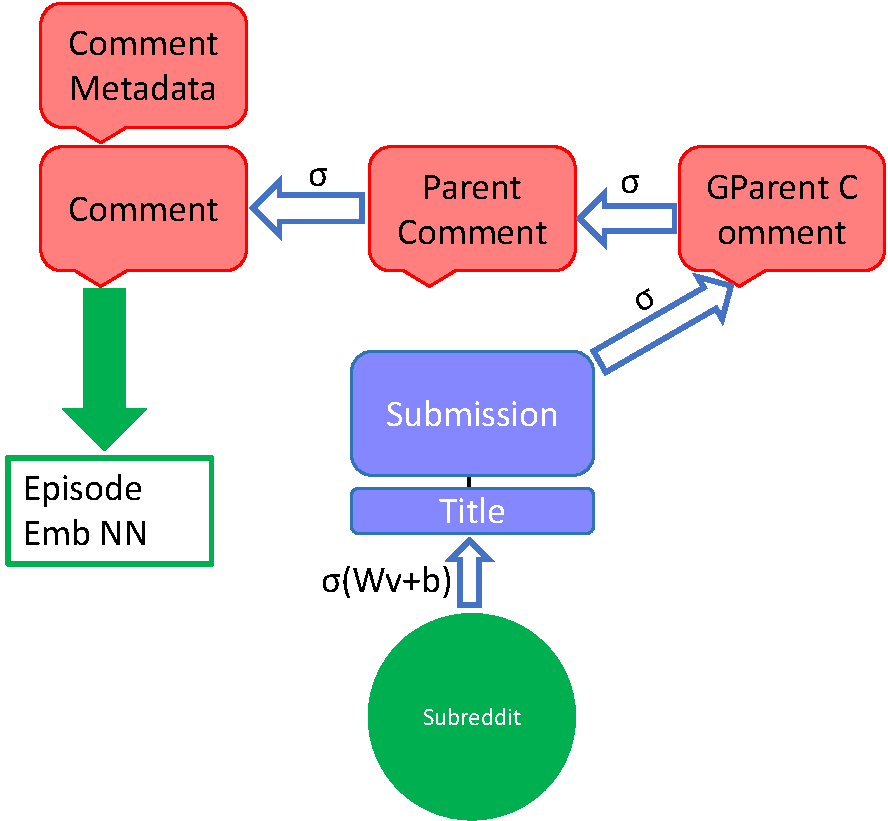
\includegraphics[width=0.5\linewidth,alt={Block diagram for context-based approach.}]{future_work/figures/reddit_context_based.pdf}
    \caption{Context based Author Identification Embedding}
    \label{fig:future_work:scale:preliminary:reddit_context_embedding}
\end{figure}
The second approach, designated as the \textit{context-based} approach uses the structure of the Reddit graph to collect surrounding context for each post prior to embedding it. 
We systematically add the context from parent nodes ((grand)parent comment, thread, subreddit), each of which are individually embedded using a shared text embedding neural network.
Each layer of the architecture adds some context before applying a non-linear transformation.
Figure~\ref{fig:future_work:scale:preliminary:reddit_context_embedding} provides a  visual representation of the transformations.

\textbf{Preliminary Results}

\begin{figure}
    \centering
    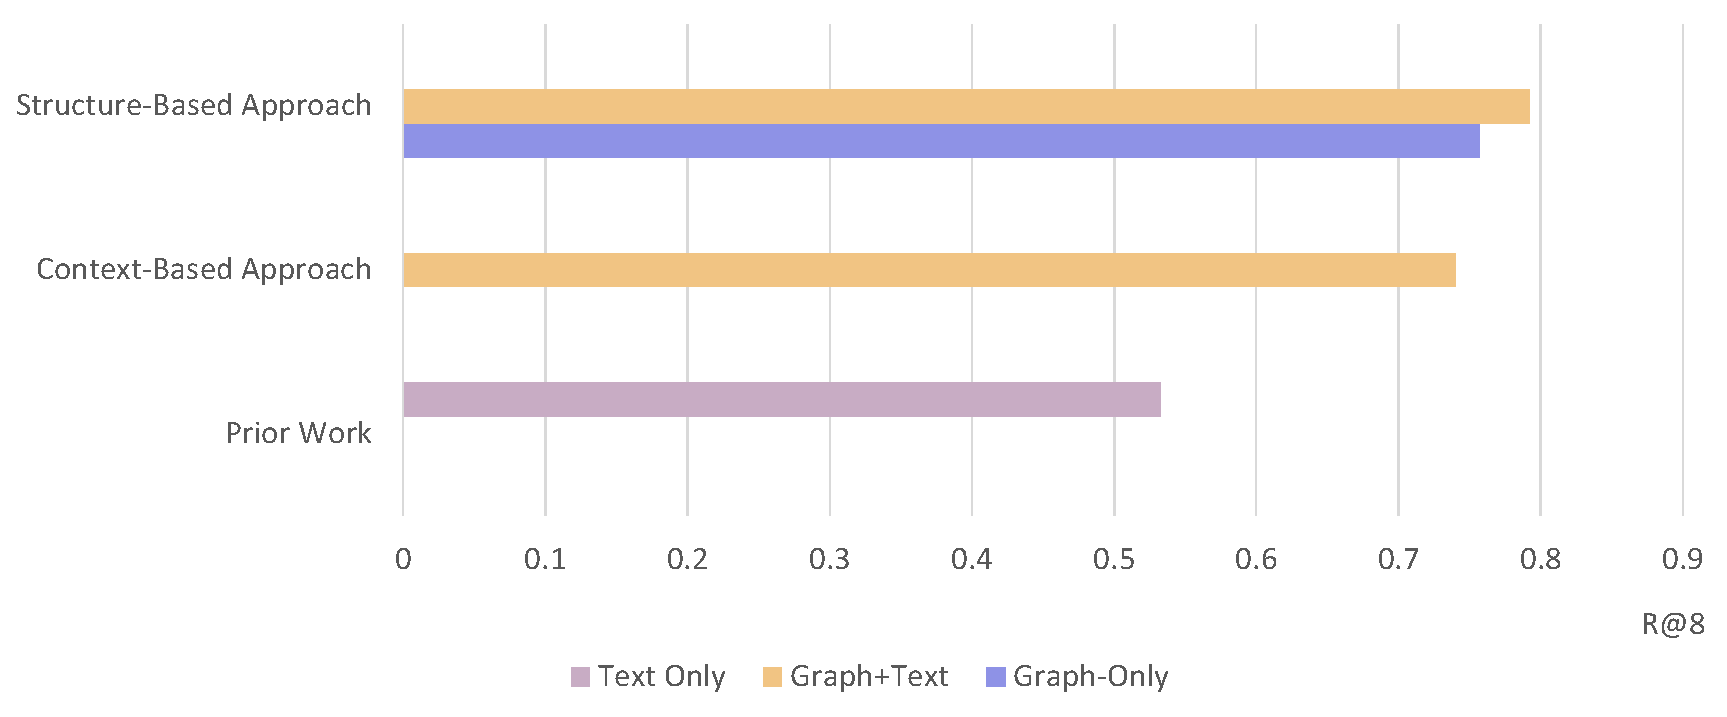
\includegraphics[width=0.8\linewidth,alt={Bar plot of preliminary results on Reddit.}]{future_work/figures/reddit_scale_graph.pdf}
    \caption{Results on author identification with preliminary approaches on a validation split. R@8 = recall at 8.}
    \label{fig:future_work:scale:preliminary:results}
\end{figure}
We test these approaches using SVDs of the adjacency matrix for structure-aware embeddings (à la \citet{agterberg2020vertex}) and text CNNs for embedding texts.
Figure~\ref{fig:future_work:scale:preliminary:results} demonstrates that these directions have the potential for improving author identification even on a large scale dataset.

\subsection{Future Directions}
The preliminary results are promising and demonstrate improvements over the text-based baseline.
In future work, we aim to explore the impact of alternative structure embeddings, including GNN based~\cite{velivckovic2018graph,hamilton2017inductive} and anonymous walk-based embeddings~\citep{ivanov2018anonymous,wang2020inductive}.
In particular, successes from scaling GraphSAGE-based~\cite{hamilton2017inductive,ying2018graph} approaches motivate their potential use in a hybrid fashion, where both the structure and text embeddings may be fused more effectively.
Additionally, the results in Figure~\ref{fig:future_work:scale:preliminary:results} are evaluated on a specific validation dataset.
Additional experiments need to be carried out to test whether the different stages (embedding, alignment) are affected by temporal shifts.
Finally, we aim to test the impact of using structure and context to help in better adaptation across different domains.
Similar to our study of domain adaptation for text embeddings (from Chapter~\ref{chp:stylometry_extensions}), we would aim to test whether structure-aware embedding would adapt to authorship identification datasets from Dread and Twitter.
%We will use datasets of Dread posts~\cite{pastrana2018crimebb} and Twitter posts~\cite{andrews2019learning} for these tasks.

\section{Fairness through Conformal Prediction}
The standard formulation for conformal prediction (Theorem~\ref{thm:CP:coverage}) provides a score-based mechanism to control for miscoverage in the prediction sets.
However, when dealing with fairness, we may want to reason over guarantees over other expressions that involve the inputs, labels, and predictions.
Such guarantees can be considered as a form of thresholded risk Control.
In the conformal setting, the Learn Then Test~\citep{angelopoulos2021learn} and conformal risk control~\citep{angelopoulos2024conformal} frameworks provide a way to control for model risks for specific classes of risk functions.
However, the Learn Then Test framework requires an IID assumption over the calibration data.
Therefore, in the following section, we will describe how conformal risk control can be used for providing fairness guarantees.
%first describe each of these frameworks and their limitations, and then provide a mechanism to construct fairness guarantees using risk control over different population subgroups.
Note that we will describe the split CP version of each of these frameworks.
\begin{comment}
\subsection{Learn Then Test for Risk Control}
The exposition in this section follows the definitions from~\citet{angelopoulos2021learn}.
Given an i.i.d calibration set $\gD_{\text{calib}} = \braces{(\vx_i, y_i)}_{i=1}^n$,
with the test $X_{n+1}, Y_{n+1}$ having the same distribution.
We have feature vectors $X_i \in \gX$ and labels/outcomes $Y_i \in \gY$, and a pretrained model $\hat{f}: \gX \rightarrow \gZ$, where $\gZ$ is the space of raw model outputs.
We will aim to infer a low dimensional thresholding parameter $\hat{\lambda}$, such that we can construct prediction sets $\gT_\lambda: \gX \rightarrow 2^{\gY}$ corresponding to every $\lambda$.
Given a risk function $L: \gY \times 2^{\gY} \rightarrow \R$, which maps the outcome and prediction set to a problem-specific risk score (e.g., accuracy, false discovery rate, false omission rate, etc.), we will aim to infer a $\hat{\lambda}$ to provide a guarantee over the risk function from the prediction set generated by $T_{\hat{\lambda}}$.
Specifically, define risk-controlling prediction sets as follows:
\begin{definition}[Risk-controlling prediction]
   Consider $\lambda \in \Lambda$ be a random variable. 
   An $(\alpha, \delta)$ risk controlling prediction $T_\lambda$ is one that satisfies $\Pr[L(Y_{n+1}, T_\lambda(X_{n+1})) \leq \alpha] \geq 1 - \delta$.
\end{definition}

The Learn-Then-Test procedure~\cite{angelopoulos2021learn} can be to construct risk-controlling prediction sets for an arbitrary risk function $L$.
The goal of the procedure is to find a subset $\hat{\Lambda} \subseteq \Lambda$ such that $T_\lambda$ is a risk-controlling prediction for all $\lambda \in \hat{\Lambda}$. 
For simplicity, define $L_\lambda = L[Y, T_\lambda(X)]$.
We provide the intuition for the construction of such a subset here, with the details available in the cited publication.
First, consider the discrete set $\Lambda = \braces{\lambda_1, \dots, \lambda_m}$ and associate the null hypothesis $H_i: L_{\lambda_i} > \alpha$ with each $\lambda_i$.
Use a finte-sample concentration inequality (typically a variation of Hoeffding) to generate p-values for each null hypothesis.
Finally, use a family-wise error rate (FWER) controlling procedure $\gF$ (e.g., Bonferroni, Holm, etc.) which takes the individual p-values to construct the set $\hat{\Lambda}$ such that $\Pr\left(\sup\limits_{\lambda \in \hat{\Lambda}}(L_{\lambda}) \leq \alpha \right) \leq 1-\delta$.
For example, if the p-values are $\braces{p_1, \dots, p_m}$, then the Bonferroni correction gives us $\hat{\Lambda} = \braces{\lambda_i: p_i \leq \frac{\delta}{m}}$.

\subsubsection{Extending Learn-Then-Test for Fairness}
Recent work on auditing fairness~\citep{singh2023brief,singh2023disparitymeasures} has focused on efficient estimation of fairness measures under the assumption of an IID calibration set.
These methods make distributional assumptions for the asymptotic behavior of certain group fairness definitions (specifically, asymptotic normality from the central limit theorem).
With the LTT procedure, we can provide a finite-sample guarantee for the fairness measure without any distributional assumption on the fairness measure/calibration set.
We outline two candidate procedures to construct fairness guarantees using the LTT procedure.
\begin{algorithm}
    \caption{DLearn-Then-Test for Direct Fairness Control}\label{alg:LTT:Direct}
    \begin{algorithmic}[1]
    \Procedure{Sparse\_k\_hop}{$k,\mathcal{B},\calib,\mathcal{D}$}
        \State $\text{A}\gets \Call{\text{Get\_Adjacency}}{\mathcal{D}}$ \Comment{Adjacency of $\mathcal{D}$, A $\in \mathbb{R}^{|\mathcal{D}|\times|\mathcal{D}|}$}
        \State $\text{path\_n}\gets \text{A[$\mathcal{B},:$]}$\Comment{path\_n $\in \mathbb{R}^{|\mathcal{B}|\times|\mathcal{D}|}$ }
        \State $\text{k\_hop}\gets \text{path\_n[$:,\calib$]}$\Comment{k\_hop $\in \mathbb{R}^{|\mathcal{B}|\times|\calib|}$ }
        \For{$n \in \{2,3,\hdots,k\}$}
            \State $\text{path\_n} \gets (\text{path\_n})\text{A}$
            \State $\text{neg\_if\_n}\gets \text{k\_hop}-\Call{\text{sgn}}{\text{path\_n[$:,\calib$]}}$\Comment{negative value $\implies$ n hops away}
            \State $\text{in\_n\_hop}\gets (\text{neg\_if\_n}<0)\times n$ \Comment{Nodes that are a min distance of n}
            \State $\text{k\_hop} \gets \text{k\_hop} + \text{in\_n\_hop}$
        \EndFor\label{khopendwhile}
        \State \textbf{return} $\text{k\_hop}$\Comment{$\forall_{i,j}\, \text{\textbf{If} dist($i,j$)}  \leq k \text{ \textbf{then} k\_hop[$i,j$]} = \text{dist}(i,j), \text{\textbf{else} k\_hop[$i,j$]}=0$}
    \EndProcedure
    \end{algorithmic}
    \end{algorithm}



Notably, the LTT procedure requires an IID assumption on the calibration set and thus, cannot be applied in the graph setting directly.
However, it can provide an alternative to \AVOIRmethodname{} for a non-online setting.
A LTT-based approach would produce statistical guarantees for a fixed calibration set and will not guarantee any asymptotic convergence.
%\pmcomment{endinput s missing}

\subsection{Conformal Risk Control}
%\input{graphConformal/fairness/conformal_risk_control}
\end{comment}

\subsection{Conformal Risk Control}

First, we define the framework of conformal risk control~\citep{angelopoulos2024conformal}.
We start from a calibration set $\gD_{\text{calib}} = \braces{(\vx_i, y_i)}_{i=1}^n$,
with exchangeability assumed for $\gD_{\text{calib}} \cup \braces{(X_{n+1}, Y_{n+1})}$.
We have feature vectors $X_i \in \gX$ and labels/outcomes $Y_i \in \gY$. % and a 
The guarantee provided by conformal prediction sets $C$ relates to miscoverage
\[
        \Pr\left[Y_{n+1} \not\in C(X_{n+1})\right] \leq \alpha
\]
Instead, consider any bounded loss function $L$ that is monotonically non-increasing with the increasing size of $C(X_{n+1})$.
Examples of such functions include accuracy, F1-score, and false negative rate.
Conformal Risk Control provides a mechanism to construct prediction sets $C$ that provide guarantees over a bounded loss function $L \in (-\infty, B]$:
\[
    \E\left[L(C(X_{n+1}), Y_{n+1})\right] \leq \alpha
\]
Suppose we have a trained model $\hat{f}: \gX \rightarrow \gZ$, where $\gZ$ is the space of raw model outputs which is used to create a function $C_\lambda(.)$ that constructs prediction sets for a given $\lambda$.
Where larger $\lambda$ correspond to more conservative prediction sets.
For example, for the TPS method discussed in Chapter~\ref{chp:graphConformal}, this would be $C_\lambda(X) = \braces{y: 1 - \hat{f}(X)_y \leq \lambda}$.
Conformal risk control provides a threshold $\hat{\lambda}$ such that $E[C_{\hat{\lambda}}] \leq \alpha$ for a given $\alpha < B$

\subsection{Fairness through Conformal Risk Control}
We can use conformal risk control to modify the outputs of a model to provide guarantees on any monotone loss function.
We provide one example below, constructing a guarantee for an expression capturing predictive parity. 

We will build a risk control guarantee for a predictive parity like term.
Consider a binary classification task where the label $y_1$ corresponds to acceptance and $y_0$ corresponds to rejection.
Consider two groups $g_0$ and $g_1$.
Define 
\[
    L_i(C_{\lambda_i}(X), Y) = \1[y_1 \not\in C_{\lambda_i}(X) \cap X \in g_i], i = 0, 1
\]
This loss function captures the points where the prediction set excludes acceptance for each group.
With increasing $\lambda$, $C_\lambda$ will include additional classes.
The possible values of $C_\lambda(X)$ as $\lambda$ increases, if the acceptance class $y_1$ has higher score would be $\emptyset, \braces{y_0}, \braces{y_0, y_1}$, which corresponds to loss values of $1, 1, 0$ respectively.
If the rejection class $y_0$ has a higher score, the possible values would be $\emptyset, \braces{y_1}, \braces{y_0, y_1}$, which corresponds to loss values of $1, 0, 0$ respectively.
In both cases, the loss function is monotonically non-increasing with the size of the prediction set.
Thus we can use conformal risk control over this set.
From risk control, we would get 
\[
    \hat{\lambda}_0 : E[L_0(C_{\hat{\lambda}_0}(X), Y)] \leq \alpha_0
\]
and 
\[
    \hat{\lambda}_1 : E[L_1(C_{\hat{\lambda}_1}(X), Y)] \leq \alpha_1
\]
Since $L$ is an indicator function, these guarantees corresponds to $\Pr[y_1 \not\in C_{\hat{\lambda}_i}(X) \cap X \in g_i] \leq \alpha_i$.
From this risk control and monotonicity of $L$, we can set $\hat{\lambda} = \max\{\hat{\lambda}_1, \hat{\lambda}_2\}$, and can provide a predictive parity-like guarantee for the model:
\[
    -\alpha_1 \leq \Pr[y_1 \not\in C_{\hat{\lambda}}(X) \cap X \in g_0] - \Pr[y_1 \not\in C_{\hat{\lambda}}(X) \cap X \in g_1] \leq \alpha_0
\]
Thus, given a calibration set and required thresholds $\alpha_0, \alpha_1$, we can use conformal risk control prediction sets to provide a fairness guarantee for the outputs produced by any black-box model.

This example shows the utility of conformal risk control to provide fair predictions.
We leave the exploration of the full gamut of fairness definitions and possible loss functions as future work

\begin{comment}

\section{Auditing in Non-iid Settings}
\label{sec:future_work:monitoring}
\pmcomment{TODO: this section}
In chapter~\ref{chp:avoir},  we described a confidence sequence based approach for monitoring fairness metrics associated with a decision-making function.
However, there are some assumptions underlying the derivations that allow \AVOIRmethodname{} to be used for monitoring.
In this extension, we aim to make the \AVOIRmethodname{} system more interactive, and generalize to more scenarios for more effective \textit{online monitoring}.

\subsection{Goals}
Our first goal is to make \AVOIRmethodname{} more interactive.
A user may want to change the specification that they monitor as requirements and regulations for specifications continue to evolve over time.
In the current implementation, an update of the specification requires monitoring from scratch after re-initializing all tracked expressions.
 We aim to enable more efficient modification of the monitored specification.  
The second goal is to make \AVOIRmethodname{} generalize to more diverse monitoring scenarios.
An important assumption for tracking terms in \AVOIRmethodname{} (from using the Adaptive Hoeffding inequality~\cite{zhao2016adaptive}) is that the underlying data generating process is stationary.
In the real world, this assumption may not hold.
The second assumption is the independence of decisions $y_i$ given an input $x_i$ , i.e., $y_i = f(x_i)$.
When the decision making function is based-on a non-parametric or graph-based model, this assumption may not hold.


\subsection{Datasets and Methods}
To accomplish our first goal and enable editing of specifications, we aim to implement a caching mechanism within \AVOIRmethodname{}.
We will cache the values of each \textit{elementary} subexpression and potentially certain other expressions that may help in deriving guarantees for new specifications.
In conjunction we will explore datasets and methods for fairness monitoring in non-stationary environments.
Recent work on monitoring of model performance metrics~\cite{ginart2022mldemon} test monitoring on three streaming datasets.
These include a non-stationary spam-detection dataset~\cite{katakis2005utility}, weather prediction dataset\footnote{\url{https://www.kaggle.com/datasets/jsphyg/weather-dataset-rattle-package}}, and a face detection dataset~\cite{wang2020masked}.
Along with a subset of thase and furthering our goals of exploring the non-independent decision setting, we will collect common graph datasets from SNAP~\cite{snapnets} and the Open Graph Benchmark~\cite{hu2020open}.
In terms of methods, we aim to explore recent work on improving uncertainty estimation in various non-independent and drift scenarios.
These include: black-box label shift detection~\cite{lipton2018detecting}, covariate shift~\cite{tibshirani2019conformal}, and general distribution free concentration confidence sets~\cite{howard2021time}. 
We will also contrast our setup against alternative fairness auditing mechanisms~\cite{yan2022active} that measure efficiency in terms of number of queried labels rather than the number of post-deployment observations. 
\end{comment}


\section{Towards More Robust Stylometry}

In chapters~\ref{chp:sysml} and~\ref{chp:stylometry_extensions}, we study the robustness of authorship attribution models across time and domains.
The methods we propose in chapter~\ref*{chp:sysml} require retraining a model with additional context provided from graph-based representations.
As seen in chapter~\ref*{chp:stylometry_extensions}, the representations learned by models trained on one domain do not always generalize well to other domains, or even within the same domain.
The robustness of these models across time and demographics varies.
We propose two potential directions of future work that are aimed at building more robust authorship attribution models viz. \emph{recalibration} and \emph{conformal prediction}.

%\subsection{Methods}

\subsection{Recalibration}
A model is said to be well calibrated if the score predicted by the model is a good estimate of the true probability of the event.
Specifically, consider a binary classification model that predicts a score $s$ for a given input.
For a well-calibrated model, 
\[
    \Pr(Y = 1 | S = s) = s
\]
The outputs of neural networks are not guaranteed to be well-calibrated~\citep{guo2017calibration}.
Exact calibration is difficult to achieve and measure, so binned versions of calibration are often used.
Reliability diagrams are used to visualize the calibration of a model, while the expected calibration error (ECE) is used to measure the calibration of a model.
This reliability diagram plots the empirical probability of the event against the predicted score across bins.
For a well-calibrated model, the empirical probability should match the predicted score, i.e, lie on the line $y = x$.
The expected calibration error is defined as
\[
    \text{ECE} = \sum_{m=1}^{M} \frac{|B_m|}{n} \left| \text{acc}(B_m) - \text{conf}(B_m) \right|
\]
where $B_m$ is the set of examples in bin $m$, $n$ is the total number of examples, $\text{acc}(B_m)$ is the accuracy of the model in bin $m$, and $\text{conf}(B_m)$ is the confidence of the model in bin $m$.
Methods such as temporal scaling, isotonic regression, and Platt scaling have been used to recalibrate the outputs of neural networks~\cite{guo2017calibration} to achieve calibration.

\begin{figure}[h]
    \centering
    \begin{subfigure}{0.48\linewidth}
    \centering
    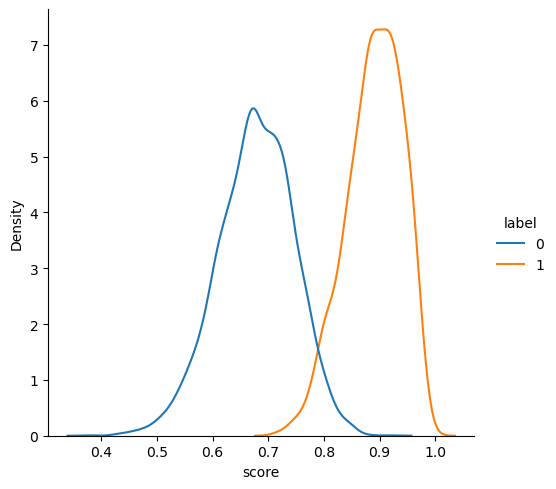
\includegraphics[width=\linewidth,alt={Density plot for calibration experiments.}]{stylometryExtensions/figures/calibration_expts/cos_dist_2015.png}
    \end{subfigure} %
    \caption{Density plot for pairwise cosine similarity for authors from the \DSvarydelta{} dataset. 1 corresponds to matching pairs, 0 corresponds to non-matching pairs.}
    \label{fig:calibration:density}
\end{figure}
For the authorship attribution task, we would aim to recalibrate the similarity scores for the representations predicted by the model so that the score is a good estimate of the true probability of the event.
We set up this problem as a binary classification task, sampling a matching pair of episodes (same author) from the query and target, and a fixed number of non-matching pairs (negative samples) for each author.
For the purpose of this discussion, we set the number of negative samples to 5.
Figure~\ref{fig:calibration:density} shows the density plot for the pairwise cosine similarity for authors from the \DSvarydelta{} dataset.
The density plot shows that the scores are separable, but it is not clear if the scores are well-calibrated.
Thus, the score could be used as a proxy for the confidence of the model in its prediction.
Other proxies may include the magnitude of the representation~\citep{novoselov2023investigation}, or estimates of error from sampling subsets of windows from an episode.
In Figure~\ref{fig:calibration:relaibility_2015}, we see that the neither the cosine similarity (cos) nor the magnitude sum (mag) are well-calibrated.
Using a logistic regression-based recalibration method, we can get a well-calibrated score for the model.

\begin{figure}
    \centering
    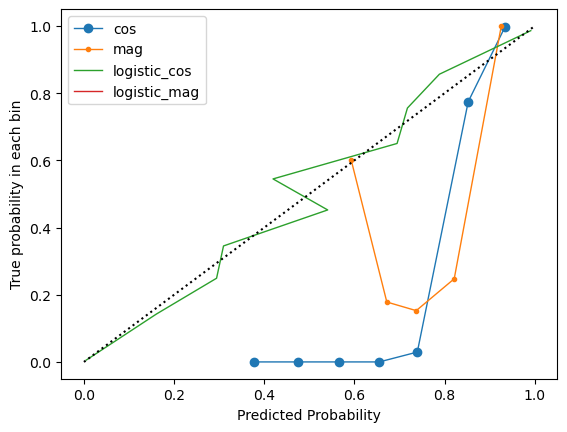
\includegraphics[width=0.7\linewidth,alt={Line plots showing reliability diagram comparisons.}]{stylometryExtensions/figures/calibration_expts/calibrate_2015.png}
    \caption{Reliability diagram for the LUAR model trained on the \DSvarydelta{} dataset for 2015. The x-axis represents the predicted score, and the y-axis represents the empirical probability of the event. The dashed line represents perfect calibration.}
    \label{fig:calibration:relaibility_2015}
\end{figure}

\begin{table}[]
\centering
\begin{tabular}{lr}
\toprule
 ECE  & year \\
\midrule
  0.003675 &2015 \\
  0.003591 &2016 \\
  0.003645 &2017 \\
  0.005089 &2018 \\
  0.007548 &2019 \\
 \bottomrule
\end{tabular}
    \caption{Measuring Temporal degradation of ECE for the recalibrated LUAR model across \DSvarydelta{} splits.}
    \label{tab:calib:init}
\end{table}

\begin{figure}
    \centering
    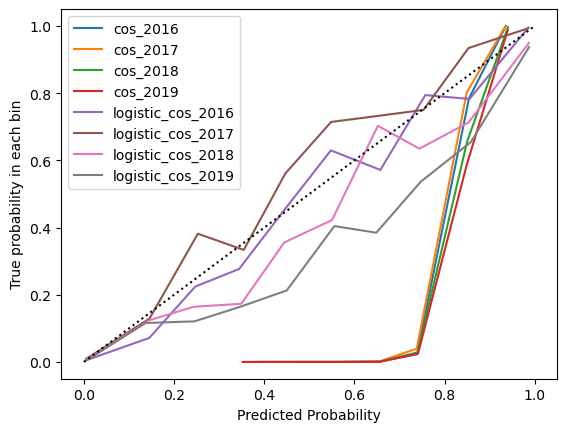
\includegraphics[width=0.8\linewidth,alt={Line plot for reliability diagram of LUAR over time.}]{stylometryExtensions/figures/calibration_expts/eval_calibration.png}
    \caption{Plots for the reliability diagrams recalibrated LUAR model across \DSvarydelta{} splits.}
    \label{fig:calibration:reliability_2016_2019}
\end{figure}

Next, we test whether this calibration displays temporal degradation.
From Figure~\ref{fig:calibration:reliability_2016_2019} and Table~\ref{tab:calib:init}, we see that the ECE is stable for a longer period but does degrade over a longer time span.
These initial experiments demonstrate that recalibration can help produce a model with more temporally robust predictions.
Further future work on recalibration may be able to achieve more robust predictions across different domains and demographics.

\subsection{Conformal Prediction}
In our work on extending runtime monitoring to graph structured data (Chapter~\ref{chp:graphConformal}), we discussed the approach of prediction sets generated through conformal prediction allowing control of the miscoverage rate.
We speculate that this may be a candidate solution for providing guarantees on the performance of authorship attribution models.
Notably, unlike the recalibration-based setup that models the task as a binary classification problem, conformal prediction could be a candidate for a more general framework for providing guarantees directly in the retrieval setting.

Specifically, a modified version of Adaptive Prediction Sets~\cite{romano2020classification} could be used to add up the scores associated with the predictions until the coverage is achieved.
Even if the threshold scores need to be recomputed, using formal guarantees provided by \citep{vovk2005algorithmic}, we can ensure that the coverage achieved is within a certain $\epsilon$ of the desired coverage.
Further, with the framework of risk control~\cite{angelopoulos2024conformal}, we can provide guarantees on the performance of the model for specific classes of risk functions.
For the case of retrieval, since we are interested in measures such as recall and MRR.
In future work, the risk control framework may be a candidate for achieving guaranteed performance for these measures.

%Our empirical results show that recalibration can be used to reduce the impact of these shifts on the performance of these models.
%However, there are no statistically sound guarantees relating the performance of the model after recalibration.
%Our success with conformal prediction in aforementioned work motivates us to use it as a tool to provide such guarantees in the context of authorship attribution.
%In the final direction of proposed future work, we discuss how a conformal prediction-based approach may be used to achieve such guarantees.
%\DSfixeddelta{}
%Steps to generate validation split for calibration:
%\begin{enumerate}
%    \item Select query/target from one split (We choose LUAR 1-15/12-15).
%    \item Calculate all pairwise cosine similarities and sum of magnitudes.
%    \item Sample a subset of users.
%    \item For each user, create a data point with label 1 and score $ = cos(f(q_{u}), f(t_{u}))$, magnitude $=\norm{f(q_{u})} + \norm{f(t_{u})}$, where $f$ is the LUAR model.
%    \item In addition, sample $n_{neg} = 5$ negative samples, with label 0 and score $ = cos(f(q_{u}), f(t_{u'}))$, magnitude $=\norm{f(q_{u})} + \norm{f(t_{u'})}$.
%    \item Make distributional plots for these (Figure~\ref{fig:calibration:density}.
%    \item Train logistic regression models which takes these (score/mag) as input and predicts the label. Create a reliability diagram for all of these models (Figure~\ref{fig:calibration:relaibility_2015}).
%    \item Plot the ROC curves corresponding to these models (Figure~\ref{fig:calibration:roc_2015})
%    \item Create similar reliability diagrams for other splits - marked degradation in calibration - room to improve (FIgure~\ref{fig:calibration:reliability_2016_2019})
%\end{enumerate}


%\begin{figure}[h]
%    \centering
%    \begin{subfigure}{0.48\linewidth}
%    \centering
%    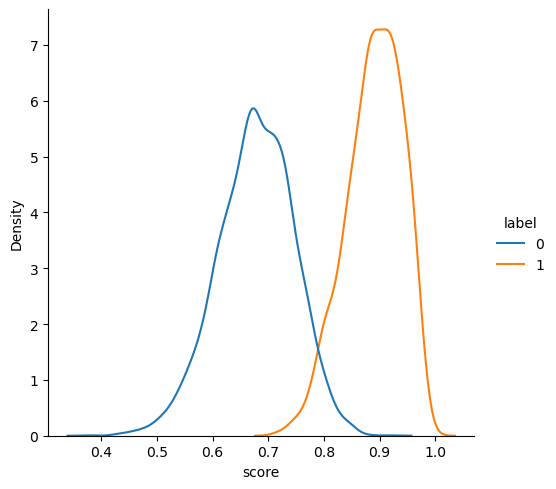
\includegraphics[width=\linewidth]{stylometryExtensions/figures/calibration_expts/cos_dist_2015.png}
%    \end{subfigure} %
%    \begin{subfigure}{0.48\linewidth}
%    \centering
%    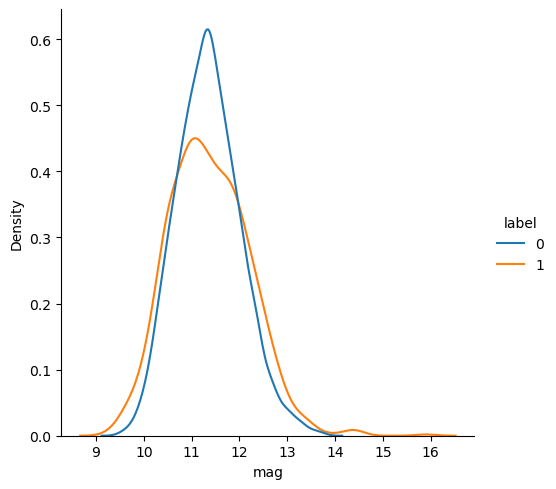
\includegraphics[width=0.5\linewidth]{stylometryExtensions/figures/calibration_expts/mag_dist_2015.png}
%    \end{subfigure} %
%    \caption{Density plots of cosine similarity (left) and magnitude sum (right).}
%    \label{fig:calibration:density}
%\end{figure}

%\begin{figure}
%    \centering
%    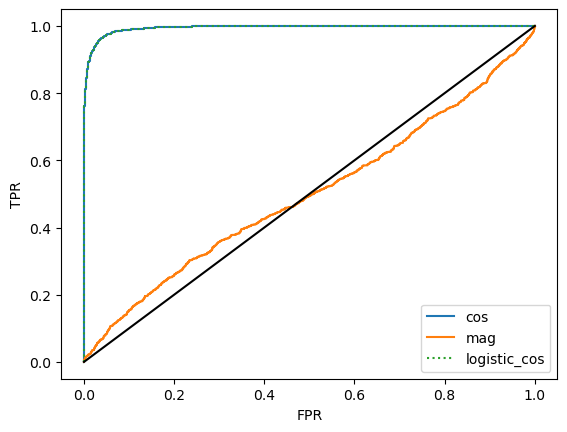
\includegraphics[width=0.5\linewidth]{stylometryExtensions/figures/calibration_expts/roc_2015.png}
%    \caption{ROC curve for LUAR 2015.}
%    \label{fig:calibration:roc_2015}
%\end{figure}



\begin{comment}
\begin{figure}
    \centering
    \includegraphics[width=\linewidth]{figures/magnitude_plots/fixeddelta_mag_density.png}
    \caption{Magnitude density plots for different splits of \DSfixeddelta{} for LUAR}
    \label{fig:temporal_fixed:magnitude:density}
\end{figure}

\begin{figure}
    \centering
    \includegraphics[width=\linewidth]{figures/magnitude_plots/fixeddelta_mag_vs_n_posts.png}
    \includegraphics[width=\linewidth]{figures/magnitude_plots/fixeddelta_mag_vs_rrank.png}
    \caption{Magnitude negatively correlated with number of posts, not correlated with reciprocal rank for \DSfixeddelta{}}
    \label{fig:temporal_fixed:manitude:density_n_posts}
\end{figure}


\begin{figure}
    \centering
    \includegraphics[width=\linewidth]{figures/magnitude_plots/varydelta_mag_density.png}
    \caption{Magnitude density plot for \DSvarydelta{}}
    \label{fig:tempral_vary:magnitude:density}
\end{figure}
\end{comment}

%\pmComment{TODO: Add a section summarizing conformal idea}


%
%\section{Interpretable Stylometric Modeling}
%\label{sec:future_work:interpret}
%In this direction of future work, we aim to build to improve the interpretability of representation learning models for authorship identification, including those that may use multiple modalities (such as graphs and text).
%In Section~\ref{sec:sysml:analysis}, we demonstrated the use of gradient-based methods as a preliminary approach for interpretation for the authorship identification task.
%However, unlike other common NLP tasks such as such as sentiment analysis, relation extraction, and question answering, stylometric evidence may not be directly associated with single spans of text.
%For example, the occurrence of spans having positive words/phrases may provide evidence for positive sentiment predictions by a machine learning model.
%This can be associated with a gradient-based explanation, for example, if the removal of this phrase would cause the model to change its output.
%However, in the authorship identification setting, the removal of a phrase from a single text may not be sufficient to change the output of a model since the phrase may continue to occur in a sufficient number of alternative posts created by the same author.
%Thus, in the \textit{episode}-based setup where we combine multiple posts by a single author, an explanation may be associated with a set of related modifications rather than a single removal.
%Exploring the contribution of different changes within a set provides a setup for exploiting \textit{structure} for interpretation.
%We propose two directions of exploration for future work.
%
%\subsection{Goals}
%Our goal is to generate explanations that are faithful to the model used for authorship attribution while also being useful for end uses of these models for decision making.
%In an ideal scenario, we would be privy to the proprietary tools used by various social media platforms such as \citet{reddit2020banevasion} and \citet{twitch2021banevasion} for content moderation, and also be able to access the justifications provided by humans when making these decisions.
%However, the tools and justifications are usually not publicly available.
%
%\subsection{Datasets and Methods}
%
%Due to the paucity of public datasets, we aim to study the Wikipedia Sockpuppet Investigation data~\cite{wiki2008SPI} and associated tools~\cite{smith2020wikipediaSPItools}, which  include publicly accessible justifications to understand the factors that are weighed by humans when making these decisions.
%Concurrently, we aim to game theoretic mechanisms for exploring \textit{structure} for explanations of machine learning models.
%These models~\cite{datta2016algorithmic,lundberg2017unified,sundararajan2020many,yan2021if} use Shapley values to generate attribution scores which are more suited for set-based explanations.
%Shapley values can be used to understand the weight of contributions of different elements of a set of changes in the output of the author identification models. 
%We will use the wikipedia sockpuppet datasets to understand the scope of modifications that can actually help in decision making, in conjunction with an \textit{adversarial testing} setup to study how different perturbations affect the value function for explanations.
%Training a model to learn the value function associated with an authorship identification model can help provide explanations that may be useful to end-users.
%
%
%\section{Project Schedule and Timeline}
%In Table~\ref{tab:future_work:timeline}, we define a plausible timeline over which we aim to accomplish the future work discussed in this section.
%The duration is aligned with The Ohio State University academic calendar.
%We anticipate that some of the work may roll-over into Spring 2024, contingent upon encountering roadblocks in the course of research.
%
%\begin{table}
%    \centering
%    \begin{tabular}{llcc}
%    \toprule
%        Project & Task & Priority & Duration  \\
%        \midrule 
%     \multirow{3}{*}{\ref{sec:future_work:scale}} & Structure + Alignment Approaches & High & Fall '22\\
%        & Context-based and Hybrid Approaches & High & Fall '22 - Spring '23 \\
%        & Cross domain experiments & Medium & Spring '22 \\
%    \midrule
%    \multirow{2}{*}{\ref{sec:future_work:interpret}} & Wikipedia sockpuppet data analysis & Medium & Summer '23 - Fall '23  \\
%    & Shapley value based explanations & Medium & Summer '23 - Fall '23\\
%    \midrule 
%    \multirow{2}{*}{\ref{sec:future_work:monitoring}} & Caching for better interaction & Medium & Summer '23 - Fall '23\\
%    & Non-IID uncertainity estimation & High & Spring '23 - Summer '23\\
%    \bottomrule
%    \end{tabular}
%    \caption{Plausible Project Schedule for Proposed Future Work.}
%    \label{tab:future_work:timeline}
%\end{table}

\endinput